\newpage
\section{Umsetzung (ca. 10 Seiten)}
Nachdem die theoretischen Grundlagen im letzten Kapitel vorgestellt wurden, wird in diesem Kapitel die Umsetzung beschrieben. Dieses Kapitel wird nach einem geordneten Vorgehen strukturiert. Zuerst werden verfügbare Daten vorgestellt, analysiert und sortiert. In diesem Schritt wird entschieden, welche Daten die Zielvariable Nachfrage beeinflussen und somit mit in das Modell eingegeben werden. Die deskriptive Analyse unterstützt dabei die Visualisierung der Daten und verleiht mehr Verständnis für den Ablauf der Media-Kanäle. Darauffolgend werden die Daten in das OLS-Modell eingesetzt. Die Ergebnisse des Modells werden analysiert.
\subsection{Einsatz der deskriptiven Analyse für die Datenbewertung}
Wie im \autoref{deskriptiveanalyse} beschrieben, fasst die deskriptive Analyse historische Daten zusammen und zeigt wichtige Muster und Trends auf. Sie bildet die Grundlage für weiterführende Analysen und datengestützte Entscheidungen. Um auf den Einsatz des OLS-Modells vorzubereiten, werden die Daten vom \ac{MMM} deskriptiv analysiert. \\\\
Zuerst werden die Daten für das \ac{MMM} ausgewertet. Für das \ac{MMM} bei bonprix werden Daten ab dem 01.01.2022 vorbereitet. Da Media ein Unterkanal des \ac{MMM}s ist, werden die \ac{MMM}-Daten auch für Media verwendet. \\\\

\begin{figure}[ht]
    \centering
    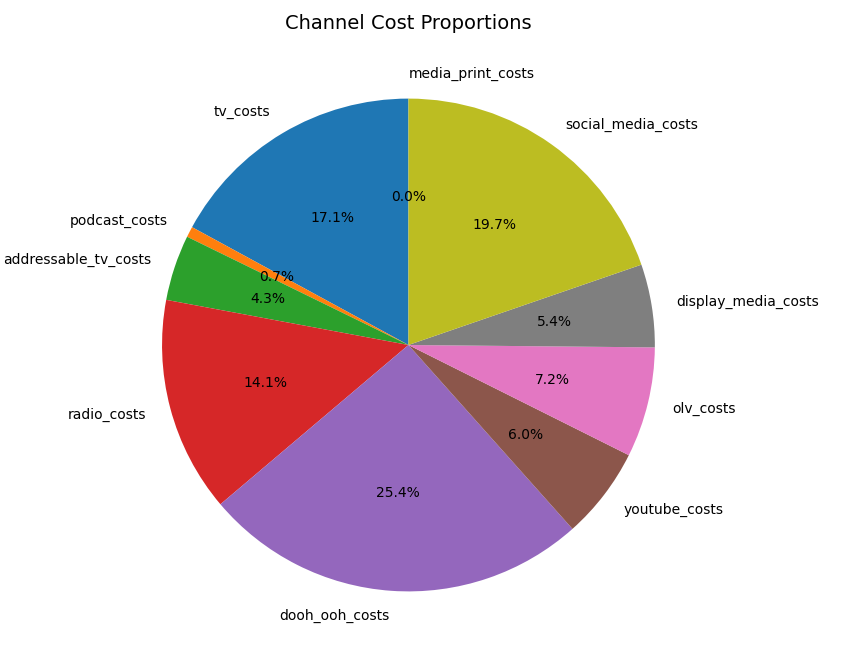
\includegraphics[width=0.8\linewidth]{images/mediapie.png}
    \caption{Kostenanteil der Media-Kanäle bei bonprix, eigene Darstellung}
    \label{fig:enter-label}
\end{figure}

\subsection{Daten auswerten}
\subsection{Einsetzung des Marketing-Mix-Modells}
\subsection{Modell-Ergebnis}
